\documentclass[twoside]{book}

% Packages required by doxygen
\usepackage{fixltx2e}
\usepackage{calc}
\usepackage{doxygen}
\usepackage[export]{adjustbox} % also loads graphicx
\usepackage{graphicx}
\usepackage[utf8]{inputenc}
\usepackage{makeidx}
\usepackage{multicol}
\usepackage{multirow}
\PassOptionsToPackage{warn}{textcomp}
\usepackage{textcomp}
\usepackage[nointegrals]{wasysym}
\usepackage[table]{xcolor}

% Font selection
\usepackage[T1]{fontenc}
\usepackage[scaled=.90]{helvet}
\usepackage{courier}
\usepackage{amssymb}
\usepackage{sectsty}
\renewcommand{\familydefault}{\sfdefault}
\allsectionsfont{%
  \fontseries{bc}\selectfont%
  \color{darkgray}%
}
\renewcommand{\DoxyLabelFont}{%
  \fontseries{bc}\selectfont%
  \color{darkgray}%
}
\newcommand{\+}{\discretionary{\mbox{\scriptsize$\hookleftarrow$}}{}{}}

% Page & text layout
\usepackage{geometry}
\geometry{%
  a4paper,%
  top=2.5cm,%
  bottom=2.5cm,%
  left=2.5cm,%
  right=2.5cm%
}
\tolerance=750
\hfuzz=15pt
\hbadness=750
\setlength{\emergencystretch}{15pt}
\setlength{\parindent}{0cm}
\setlength{\parskip}{3ex plus 2ex minus 2ex}
\makeatletter
\renewcommand{\paragraph}{%
  \@startsection{paragraph}{4}{0ex}{-1.0ex}{1.0ex}{%
    \normalfont\normalsize\bfseries\SS@parafont%
  }%
}
\renewcommand{\subparagraph}{%
  \@startsection{subparagraph}{5}{0ex}{-1.0ex}{1.0ex}{%
    \normalfont\normalsize\bfseries\SS@subparafont%
  }%
}
\makeatother

% Headers & footers
\usepackage{fancyhdr}
\pagestyle{fancyplain}
\fancyhead[LE]{\fancyplain{}{\bfseries\thepage}}
\fancyhead[CE]{\fancyplain{}{}}
\fancyhead[RE]{\fancyplain{}{\bfseries\leftmark}}
\fancyhead[LO]{\fancyplain{}{\bfseries\rightmark}}
\fancyhead[CO]{\fancyplain{}{}}
\fancyhead[RO]{\fancyplain{}{\bfseries\thepage}}
\fancyfoot[LE]{\fancyplain{}{}}
\fancyfoot[CE]{\fancyplain{}{}}
\fancyfoot[RE]{\fancyplain{}{\bfseries\scriptsize Generated by Doxygen }}
\fancyfoot[LO]{\fancyplain{}{\bfseries\scriptsize Generated by Doxygen }}
\fancyfoot[CO]{\fancyplain{}{}}
\fancyfoot[RO]{\fancyplain{}{}}
\renewcommand{\footrulewidth}{0.4pt}
\renewcommand{\chaptermark}[1]{%
  \markboth{#1}{}%
}
\renewcommand{\sectionmark}[1]{%
  \markright{\thesection\ #1}%
}

% Indices & bibliography
\usepackage{natbib}
\usepackage[titles]{tocloft}
\setcounter{tocdepth}{3}
\setcounter{secnumdepth}{5}
\makeindex

% Hyperlinks (required, but should be loaded last)
\usepackage{ifpdf}
\ifpdf
  \usepackage[pdftex,pagebackref=true]{hyperref}
\else
  \usepackage[ps2pdf,pagebackref=true]{hyperref}
\fi
\hypersetup{%
  colorlinks=true,%
  linkcolor=blue,%
  citecolor=blue,%
  unicode%
}

% Custom commands
\newcommand{\clearemptydoublepage}{%
  \newpage{\pagestyle{empty}\cleardoublepage}%
}

\usepackage{caption}
\captionsetup{labelsep=space,justification=centering,font={bf},singlelinecheck=off,skip=4pt,position=top}

%===== C O N T E N T S =====

\begin{document}

% Titlepage & ToC
\hypersetup{pageanchor=false,
             bookmarksnumbered=true,
             pdfencoding=unicode
            }
\pagenumbering{roman}
\begin{titlepage}
\vspace*{7cm}
\begin{center}%
{\Large Turtlebot\+\_\+\+Walker }\\
\vspace*{1cm}
{\large Generated by Doxygen 1.8.11}\\
\end{center}
\end{titlepage}
\clearemptydoublepage
\tableofcontents
\clearemptydoublepage
\pagenumbering{arabic}
\hypersetup{pageanchor=true}

%--- Begin generated contents ---
\chapter{Build procedures\+:}
\label{md_readme}
\hypertarget{md_readme}{}

\begin{DoxyEnumerate}
\item Clone turtlebot\+\_\+walker branch from github by inputting 
\begin{DoxyCode}
1 git clone -b turtlebot\_walker https://github.com/yhsueh/beginner\_tutorials.git
\end{DoxyCode}

\item Move beginner\+\_\+tutorials into src folder in your catkin\+\_\+ws.
\end{DoxyEnumerate}
\begin{DoxyEnumerate}
\item Make sure R\+O\+S\+\_\+\+P\+A\+C\+K\+A\+G\+E\+\_\+\+P\+A\+TH enviroment variable contain the workspace folder. This is done by sourcing the generated setup file under devel folder in the parent directory.
\item Input 
\begin{DoxyCode}
1 catkin\_make
\end{DoxyCode}
 to build the R\+OS package.
\end{DoxyEnumerate}

\subsection*{Procedures for running the turtlebot simulation\+:}


\begin{DoxyEnumerate}
\item Run roslaunch file to start gazebo, and two necessary nodes. 
\begin{DoxyCode}
1 roslaunch turtlebot\_walker turtlebot\_world.launch
\end{DoxyCode}
 The simulation can be recorded if record\+\_\+flag is set to 1; 
\begin{DoxyCode}
1 roslaunch turtlebot\_walker turtlebot\_world.launch record\_flag:=1
\end{DoxyCode}

\item Switch back to gazebo and view the simulation.
\item See what topics is recorded 
\begin{DoxyCode}
1 cd \{"turtlebot\_walker"\}/results
2 rosbag info bagfile.bag
\end{DoxyCode}
 
\end{DoxyEnumerate}
\chapter{Class Index}
\section{Class List}
Here are the classes, structs, unions and interfaces with brief descriptions\+:\begin{DoxyCompactList}
\item\contentsline{section}{\hyperlink{classLaserCallback}{Laser\+Callback} }{\pageref{classLaserCallback}}{}
\end{DoxyCompactList}

\chapter{File Index}
\section{File List}
Here is a list of all files with brief descriptions\+:\begin{DoxyCompactList}
\item\contentsline{section}{include/\hyperlink{LaserCallback_8hpp}{Laser\+Callback.\+hpp} \\*This class is responsible for the callback from the scan topic of the depthimage\+\_\+to\+\_\+laserscan node. It also returns the motion mode which is a boolean value }{\pageref{LaserCallback_8hpp}}{}
\item\contentsline{section}{src/\hyperlink{LaserCallback_8cpp}{Laser\+Callback.\+cpp} \\*The implementation of \hyperlink{classLaserCallback}{Laser\+Callback} class }{\pageref{LaserCallback_8cpp}}{}
\item\contentsline{section}{src/\hyperlink{laserReading_8cpp}{laser\+Reading.\+cpp} \\*This node takes and analyze the range data. Subsequently, pass the the decision made based on the data to the turtle\+Ctrl node which manipulates the turtlebot }{\pageref{laserReading_8cpp}}{}
\item\contentsline{section}{src/\hyperlink{turtleCtrl_8cpp}{turtle\+Ctrl.\+cpp} \\*The velocity commanding node. It takes the decision made from the laser\+Reading node and pass the velocities message to the turtlebot }{\pageref{turtleCtrl_8cpp}}{}
\end{DoxyCompactList}

\chapter{Class Documentation}
\hypertarget{classLaserCallback}{}\section{Laser\+Callback Class Reference}
\label{classLaserCallback}\index{Laser\+Callback@{Laser\+Callback}}


{\ttfamily \#include $<$Laser\+Callback.\+hpp$>$}

\subsection*{Public Member Functions}
\begin{DoxyCompactItemize}
\item 
\hyperlink{classLaserCallback_ab3c530049c01190fcb107019cd36c256}{Laser\+Callback} ()=default
\item 
void \hyperlink{classLaserCallback_ac721e42c1d2d3de0d1eff3ff1134544e}{callback} (const sensor\+\_\+msgs\+::\+Laser\+Scan\+::\+Const\+Ptr \&\hyperlink{turtleCtrl_8cpp_aba2f97176e275688941f5c2a40324b8a}{msg})
\item 
bool \hyperlink{classLaserCallback_ad5caf1c0a4d7f6bb87c61a59b6f1d3b5}{motion\+Mode} ()
\end{DoxyCompactItemize}
\subsection*{Public Attributes}
\begin{DoxyCompactItemize}
\item 
float \hyperlink{classLaserCallback_a0405af031c7694991b9b32f5956cbc36}{minimal} = 10
\end{DoxyCompactItemize}


\subsection{Constructor \& Destructor Documentation}
\index{Laser\+Callback@{Laser\+Callback}!Laser\+Callback@{Laser\+Callback}}
\index{Laser\+Callback@{Laser\+Callback}!Laser\+Callback@{Laser\+Callback}}
\subsubsection[{\texorpdfstring{Laser\+Callback()=default}{LaserCallback()=default}}]{\setlength{\rightskip}{0pt plus 5cm}Laser\+Callback\+::\+Laser\+Callback (
\begin{DoxyParamCaption}
{}
\end{DoxyParamCaption}
)\hspace{0.3cm}{\ttfamily [default]}}\hypertarget{classLaserCallback_ab3c530049c01190fcb107019cd36c256}{}\label{classLaserCallback_ab3c530049c01190fcb107019cd36c256}


\subsection{Member Function Documentation}
\index{Laser\+Callback@{Laser\+Callback}!callback@{callback}}
\index{callback@{callback}!Laser\+Callback@{Laser\+Callback}}
\subsubsection[{\texorpdfstring{callback(const sensor\+\_\+msgs\+::\+Laser\+Scan\+::\+Const\+Ptr \&msg)}{callback(const sensor_msgs::LaserScan::ConstPtr &msg)}}]{\setlength{\rightskip}{0pt plus 5cm}void Laser\+Callback\+::callback (
\begin{DoxyParamCaption}
\item[{const sensor\+\_\+msgs\+::\+Laser\+Scan\+::\+Const\+Ptr \&}]{msg}
\end{DoxyParamCaption}
)}\hypertarget{classLaserCallback_ac721e42c1d2d3de0d1eff3ff1134544e}{}\label{classLaserCallback_ac721e42c1d2d3de0d1eff3ff1134544e}
Handling callback

Find the least distance from the laser range data. \index{Laser\+Callback@{Laser\+Callback}!motion\+Mode@{motion\+Mode}}
\index{motion\+Mode@{motion\+Mode}!Laser\+Callback@{Laser\+Callback}}
\subsubsection[{\texorpdfstring{motion\+Mode()}{motionMode()}}]{\setlength{\rightskip}{0pt plus 5cm}bool Laser\+Callback\+::motion\+Mode (
\begin{DoxyParamCaption}
{}
\end{DoxyParamCaption}
)}\hypertarget{classLaserCallback_ad5caf1c0a4d7f6bb87c61a59b6f1d3b5}{}\label{classLaserCallback_ad5caf1c0a4d7f6bb87c61a59b6f1d3b5}
1 means there is not obstacles ahead, and 0 otherwise.

Set the motion mode. 1 when the path is clear. 0 when obstacles present. 

\subsection{Member Data Documentation}
\index{Laser\+Callback@{Laser\+Callback}!minimal@{minimal}}
\index{minimal@{minimal}!Laser\+Callback@{Laser\+Callback}}
\subsubsection[{\texorpdfstring{minimal}{minimal}}]{\setlength{\rightskip}{0pt plus 5cm}float Laser\+Callback\+::minimal = 10}\hypertarget{classLaserCallback_a0405af031c7694991b9b32f5956cbc36}{}\label{classLaserCallback_a0405af031c7694991b9b32f5956cbc36}
The minimal distance from the range measurments 

The documentation for this class was generated from the following files\+:\begin{DoxyCompactItemize}
\item 
include/\hyperlink{LaserCallback_8hpp}{Laser\+Callback.\+hpp}\item 
src/\hyperlink{LaserCallback_8cpp}{Laser\+Callback.\+cpp}\end{DoxyCompactItemize}

\chapter{File Documentation}
\hypertarget{CMakeLists_8txt}{}\section{C\+Make\+Lists.\+txt File Reference}
\label{CMakeLists_8txt}\index{C\+Make\+Lists.\+txt@{C\+Make\+Lists.\+txt}}

\hypertarget{LaserCallback_8hpp}{}\section{include/\+Laser\+Callback.hpp File Reference}
\label{LaserCallback_8hpp}\index{include/\+Laser\+Callback.\+hpp@{include/\+Laser\+Callback.\+hpp}}


This class is responsible for the callback from the scan topic of the depthimage\+\_\+to\+\_\+laserscan node. It also returns the motion mode which is a boolean value.  


{\ttfamily \#include \char`\"{}ros/ros.\+h\char`\"{}}\\*
{\ttfamily \#include \char`\"{}sensor\+\_\+msgs/\+Laser\+Scan.\+h\char`\"{}}\\*
Include dependency graph for Laser\+Callback.\+hpp\+:
\nopagebreak
\begin{figure}[H]
\begin{center}
\leavevmode
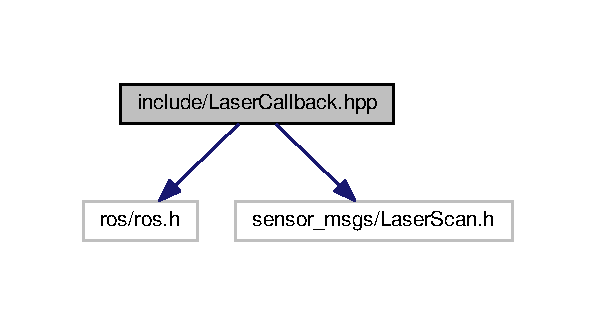
\includegraphics[width=286pt]{LaserCallback_8hpp__incl}
\end{center}
\end{figure}
This graph shows which files directly or indirectly include this file\+:
\nopagebreak
\begin{figure}[H]
\begin{center}
\leavevmode
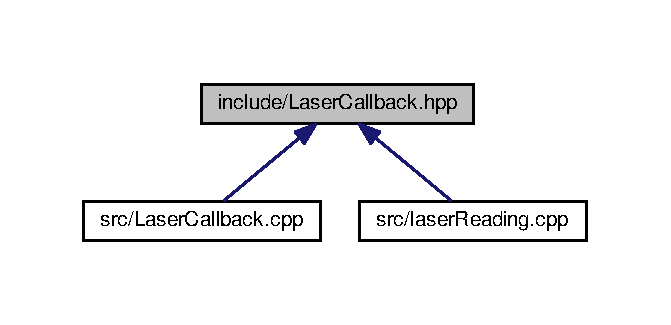
\includegraphics[width=322pt]{LaserCallback_8hpp__dep__incl}
\end{center}
\end{figure}
\subsection*{Classes}
\begin{DoxyCompactItemize}
\item 
class \hyperlink{classLaserCallback}{Laser\+Callback}
\end{DoxyCompactItemize}


\subsection{Detailed Description}
This class is responsible for the callback from the scan topic of the depthimage\+\_\+to\+\_\+laserscan node. It also returns the motion mode which is a boolean value. 


\hypertarget{license_8txt}{}\section{license.\+txt File Reference}
\label{license_8txt}\index{license.\+txt@{license.\+txt}}
\subsection*{Functions}
\begin{DoxyCompactItemize}
\item 
Copyright Yuyu\+Hsueh Redistribution and use in source and binary with or without are permitted provided that the following conditions are this list of conditions and the following disclaimer Redistributions in binary form must reproduce the above copyright this list of conditions and the following disclaimer in the documentation and or other materials provided with the distribution Neither the name of the copyright holder nor the names of its contributors may be used to endorse or promote products derived from this software without specific prior written permission T\+H\+IS S\+O\+F\+T\+W\+A\+RE IS P\+R\+O\+V\+I\+D\+ED BY T\+HE C\+O\+P\+Y\+R\+I\+G\+HT H\+O\+L\+D\+E\+RS A\+ND C\+O\+N\+T\+R\+I\+B\+U\+T\+O\+RS AS IS A\+ND A\+NY E\+X\+P\+R\+E\+SS OR I\+M\+P\+L\+I\+ED B\+UT N\+OT L\+I\+M\+I\+T\+ED T\+HE I\+M\+P\+L\+I\+ED \hyperlink{license_8txt_a042eb66328050ad88743187ae8e43b95}{W\+A\+R\+R\+A\+N\+T\+I\+ES} OF M\+E\+R\+C\+H\+A\+N\+T\+A\+B\+I\+L\+I\+TY A\+ND F\+I\+T\+N\+E\+SS F\+OR A P\+A\+R\+T\+I\+C\+U\+L\+AR P\+U\+R\+P\+O\+SE A\+RE D\+I\+S\+C\+L\+A\+I\+M\+ED IN NO E\+V\+E\+NT S\+H\+A\+LL T\+HE C\+O\+P\+Y\+R\+I\+G\+HT H\+O\+L\+D\+ER OR C\+O\+N\+T\+R\+I\+B\+U\+T\+O\+RS BE L\+I\+A\+B\+LE F\+OR A\+NY OR C\+O\+N\+S\+E\+Q\+U\+E\+N\+T\+I\+AL \hyperlink{license_8txt_aef6a70d7e2ff0800bdd6b6c943108868}{D\+A\+M\+A\+G\+ES} (\hyperlink{license_8txt_ac6699313e23a90e93d8db75154e2e689}{I\+N\+C\+L\+U\+D\+I\+NG}, B\+UT N\+OT L\+I\+M\+I\+T\+ED \hyperlink{license_8txt_a4bddb9a7dc45727be85d1869ee6c870d}{TO}, P\+R\+O\+C\+U\+R\+E\+M\+E\+NT OF S\+U\+B\+S\+T\+I\+T\+U\+TE G\+O\+O\+DS OR S\+E\+R\+V\+I\+C\+ES;L\+O\+SS OF U\+SE, D\+A\+TA, OR P\+R\+O\+F\+I\+TS;OR B\+U\+S\+I\+N\+E\+SS I\+N\+T\+E\+R\+R\+U\+P\+T\+I\+ON) H\+O\+W\+E\+V\+ER C\+A\+U\+S\+ED A\+ND ON A\+NY T\+H\+E\+O\+RY OF \hyperlink{license_8txt_a293cddb201641aed1186322968630e55}{L\+I\+A\+B\+I\+L\+I\+TY}
\item 
Copyright Yuyu\+Hsueh Redistribution and use in source and binary with or without are permitted provided that the following conditions are this list of conditions and the following disclaimer Redistributions in binary form must reproduce the above copyright this list of conditions and the following disclaimer in the documentation and or other materials provided with the distribution Neither the name of the copyright holder nor the names of its contributors may be used to endorse or promote products derived from this software without specific prior written permission T\+H\+IS S\+O\+F\+T\+W\+A\+RE IS P\+R\+O\+V\+I\+D\+ED BY T\+HE C\+O\+P\+Y\+R\+I\+G\+HT H\+O\+L\+D\+E\+RS A\+ND C\+O\+N\+T\+R\+I\+B\+U\+T\+O\+RS AS IS A\+ND A\+NY E\+X\+P\+R\+E\+SS OR I\+M\+P\+L\+I\+ED B\+UT N\+OT L\+I\+M\+I\+T\+ED T\+HE I\+M\+P\+L\+I\+ED \hyperlink{license_8txt_a042eb66328050ad88743187ae8e43b95}{W\+A\+R\+R\+A\+N\+T\+I\+ES} OF M\+E\+R\+C\+H\+A\+N\+T\+A\+B\+I\+L\+I\+TY A\+ND F\+I\+T\+N\+E\+SS F\+OR A P\+A\+R\+T\+I\+C\+U\+L\+AR P\+U\+R\+P\+O\+SE A\+RE D\+I\+S\+C\+L\+A\+I\+M\+ED IN NO E\+V\+E\+NT S\+H\+A\+LL T\+HE C\+O\+P\+Y\+R\+I\+G\+HT H\+O\+L\+D\+ER OR C\+O\+N\+T\+R\+I\+B\+U\+T\+O\+RS BE L\+I\+A\+B\+LE F\+OR A\+NY OR C\+O\+N\+S\+E\+Q\+U\+E\+N\+T\+I\+AL W\+H\+E\+T\+H\+ER IN S\+T\+R\+I\+CT OR \hyperlink{license_8txt_a053f3866e9a0ed6d815ff119b776cf19}{T\+O\+RT} (\hyperlink{license_8txt_ac6699313e23a90e93d8db75154e2e689}{I\+N\+C\+L\+U\+D\+I\+NG} N\+E\+G\+L\+I\+G\+E\+N\+CE OR O\+T\+H\+E\+R\+W\+I\+SE) A\+R\+I\+S\+I\+NG IN A\+NY W\+AY O\+UT OF T\+HE U\+SE OF T\+H\+IS S\+O\+F\+T\+W\+A\+RE
\end{DoxyCompactItemize}
\subsection*{Variables}
\begin{DoxyCompactItemize}
\item 
Copyright Yuyu\+Hsueh Redistribution and use in source and binary \hyperlink{license_8txt_a907462b7b3ae0a9072f23e05f66fb7f1}{forms}
\item 
Copyright Yuyu\+Hsueh Redistribution and use in source and binary with or without \hyperlink{license_8txt_ad26192e5b2b1fdec8883d2c0110e35c6}{modification}
\item 
Copyright Yuyu\+Hsueh Redistribution and use in source and binary with or without are permitted provided that the following conditions are \hyperlink{license_8txt_ac8582a50364a60dd4d7d7d24f725c413}{met}
\item 
Copyright Yuyu\+Hsueh Redistribution and use in source and binary with or without are permitted provided that the following conditions are this list of conditions and the following disclaimer Redistributions in binary form must reproduce the above copyright \hyperlink{license_8txt_af4bbea5cb99610e4ef2a43c12b41e9c9}{notice}
\item 
Copyright Yuyu\+Hsueh Redistribution and use in source and binary with or without are permitted provided that the following conditions are this list of conditions and the following disclaimer Redistributions in binary form must reproduce the above copyright this list of conditions and the following disclaimer in the documentation and or other materials provided with the distribution Neither the name of the copyright holder nor the names of its contributors may be used to endorse or promote products derived from this software without specific prior written permission T\+H\+IS S\+O\+F\+T\+W\+A\+RE IS P\+R\+O\+V\+I\+D\+ED BY T\+HE C\+O\+P\+Y\+R\+I\+G\+HT H\+O\+L\+D\+E\+RS A\+ND C\+O\+N\+T\+R\+I\+B\+U\+T\+O\+RS AS IS A\+ND A\+NY E\+X\+P\+R\+E\+SS OR I\+M\+P\+L\+I\+ED \hyperlink{license_8txt_a042eb66328050ad88743187ae8e43b95}{W\+A\+R\+R\+A\+N\+T\+I\+ES}
\item 
Copyright Yuyu\+Hsueh Redistribution and use in source and binary with or without are permitted provided that the following conditions are this list of conditions and the following disclaimer Redistributions in binary form must reproduce the above copyright this list of conditions and the following disclaimer in the documentation and or other materials provided with the distribution Neither the name of the copyright holder nor the names of its contributors may be used to endorse or promote products derived from this software without specific prior written permission T\+H\+IS S\+O\+F\+T\+W\+A\+RE IS P\+R\+O\+V\+I\+D\+ED BY T\+HE C\+O\+P\+Y\+R\+I\+G\+HT H\+O\+L\+D\+E\+RS A\+ND C\+O\+N\+T\+R\+I\+B\+U\+T\+O\+RS AS IS A\+ND A\+NY E\+X\+P\+R\+E\+SS OR I\+M\+P\+L\+I\+ED \hyperlink{license_8txt_ac6699313e23a90e93d8db75154e2e689}{I\+N\+C\+L\+U\+D\+I\+NG}
\item 
Copyright Yuyu\+Hsueh Redistribution and use in source and binary with or without are permitted provided that the following conditions are this list of conditions and the following disclaimer Redistributions in binary form must reproduce the above copyright this list of conditions and the following disclaimer in the documentation and or other materials provided with the distribution Neither the name of the copyright holder nor the names of its contributors may be used to endorse or promote products derived from this software without specific prior written permission T\+H\+IS S\+O\+F\+T\+W\+A\+RE IS P\+R\+O\+V\+I\+D\+ED BY T\+HE C\+O\+P\+Y\+R\+I\+G\+HT H\+O\+L\+D\+E\+RS A\+ND C\+O\+N\+T\+R\+I\+B\+U\+T\+O\+RS AS IS A\+ND A\+NY E\+X\+P\+R\+E\+SS OR I\+M\+P\+L\+I\+ED B\+UT N\+OT L\+I\+M\+I\+T\+ED \hyperlink{license_8txt_a4bddb9a7dc45727be85d1869ee6c870d}{TO}
\item 
Copyright Yuyu\+Hsueh Redistribution and use in source and binary with or without are permitted provided that the following conditions are this list of conditions and the following disclaimer Redistributions in binary form must reproduce the above copyright this list of conditions and the following disclaimer in the documentation and or other materials provided with the distribution Neither the name of the copyright holder nor the names of its contributors may be used to endorse or promote products derived from this software without specific prior written permission T\+H\+IS S\+O\+F\+T\+W\+A\+RE IS P\+R\+O\+V\+I\+D\+ED BY T\+HE C\+O\+P\+Y\+R\+I\+G\+HT H\+O\+L\+D\+E\+RS A\+ND C\+O\+N\+T\+R\+I\+B\+U\+T\+O\+RS AS IS A\+ND A\+NY E\+X\+P\+R\+E\+SS OR I\+M\+P\+L\+I\+ED B\+UT N\+OT L\+I\+M\+I\+T\+ED T\+HE I\+M\+P\+L\+I\+ED \hyperlink{license_8txt_a042eb66328050ad88743187ae8e43b95}{W\+A\+R\+R\+A\+N\+T\+I\+ES} OF M\+E\+R\+C\+H\+A\+N\+T\+A\+B\+I\+L\+I\+TY A\+ND F\+I\+T\+N\+E\+SS F\+OR A P\+A\+R\+T\+I\+C\+U\+L\+AR P\+U\+R\+P\+O\+SE A\+RE D\+I\+S\+C\+L\+A\+I\+M\+ED IN NO E\+V\+E\+NT S\+H\+A\+LL T\+HE C\+O\+P\+Y\+R\+I\+G\+HT H\+O\+L\+D\+ER OR C\+O\+N\+T\+R\+I\+B\+U\+T\+O\+RS BE L\+I\+A\+B\+LE F\+OR A\+NY \hyperlink{license_8txt_a9ecfdaf89f3cf85421feb43ef16f372d}{D\+I\+R\+E\+CT}
\item 
Copyright Yuyu\+Hsueh Redistribution and use in source and binary with or without are permitted provided that the following conditions are this list of conditions and the following disclaimer Redistributions in binary form must reproduce the above copyright this list of conditions and the following disclaimer in the documentation and or other materials provided with the distribution Neither the name of the copyright holder nor the names of its contributors may be used to endorse or promote products derived from this software without specific prior written permission T\+H\+IS S\+O\+F\+T\+W\+A\+RE IS P\+R\+O\+V\+I\+D\+ED BY T\+HE C\+O\+P\+Y\+R\+I\+G\+HT H\+O\+L\+D\+E\+RS A\+ND C\+O\+N\+T\+R\+I\+B\+U\+T\+O\+RS AS IS A\+ND A\+NY E\+X\+P\+R\+E\+SS OR I\+M\+P\+L\+I\+ED B\+UT N\+OT L\+I\+M\+I\+T\+ED T\+HE I\+M\+P\+L\+I\+ED \hyperlink{license_8txt_a042eb66328050ad88743187ae8e43b95}{W\+A\+R\+R\+A\+N\+T\+I\+ES} OF M\+E\+R\+C\+H\+A\+N\+T\+A\+B\+I\+L\+I\+TY A\+ND F\+I\+T\+N\+E\+SS F\+OR A P\+A\+R\+T\+I\+C\+U\+L\+AR P\+U\+R\+P\+O\+SE A\+RE D\+I\+S\+C\+L\+A\+I\+M\+ED IN NO E\+V\+E\+NT S\+H\+A\+LL T\+HE C\+O\+P\+Y\+R\+I\+G\+HT H\+O\+L\+D\+ER OR C\+O\+N\+T\+R\+I\+B\+U\+T\+O\+RS BE L\+I\+A\+B\+LE F\+OR A\+NY \hyperlink{license_8txt_a8c44c311e30c2c13cd7035f237993b51}{I\+N\+D\+I\+R\+E\+CT}
\item 
Copyright Yuyu\+Hsueh Redistribution and use in source and binary with or without are permitted provided that the following conditions are this list of conditions and the following disclaimer Redistributions in binary form must reproduce the above copyright this list of conditions and the following disclaimer in the documentation and or other materials provided with the distribution Neither the name of the copyright holder nor the names of its contributors may be used to endorse or promote products derived from this software without specific prior written permission T\+H\+IS S\+O\+F\+T\+W\+A\+RE IS P\+R\+O\+V\+I\+D\+ED BY T\+HE C\+O\+P\+Y\+R\+I\+G\+HT H\+O\+L\+D\+E\+RS A\+ND C\+O\+N\+T\+R\+I\+B\+U\+T\+O\+RS AS IS A\+ND A\+NY E\+X\+P\+R\+E\+SS OR I\+M\+P\+L\+I\+ED B\+UT N\+OT L\+I\+M\+I\+T\+ED T\+HE I\+M\+P\+L\+I\+ED \hyperlink{license_8txt_a042eb66328050ad88743187ae8e43b95}{W\+A\+R\+R\+A\+N\+T\+I\+ES} OF M\+E\+R\+C\+H\+A\+N\+T\+A\+B\+I\+L\+I\+TY A\+ND F\+I\+T\+N\+E\+SS F\+OR A P\+A\+R\+T\+I\+C\+U\+L\+AR P\+U\+R\+P\+O\+SE A\+RE D\+I\+S\+C\+L\+A\+I\+M\+ED IN NO E\+V\+E\+NT S\+H\+A\+LL T\+HE C\+O\+P\+Y\+R\+I\+G\+HT H\+O\+L\+D\+ER OR C\+O\+N\+T\+R\+I\+B\+U\+T\+O\+RS BE L\+I\+A\+B\+LE F\+OR A\+NY \hyperlink{license_8txt_a6fe13299500a9a6c4af4434723e6afae}{I\+N\+C\+I\+D\+E\+N\+T\+AL}
\item 
Copyright Yuyu\+Hsueh Redistribution and use in source and binary with or without are permitted provided that the following conditions are this list of conditions and the following disclaimer Redistributions in binary form must reproduce the above copyright this list of conditions and the following disclaimer in the documentation and or other materials provided with the distribution Neither the name of the copyright holder nor the names of its contributors may be used to endorse or promote products derived from this software without specific prior written permission T\+H\+IS S\+O\+F\+T\+W\+A\+RE IS P\+R\+O\+V\+I\+D\+ED BY T\+HE C\+O\+P\+Y\+R\+I\+G\+HT H\+O\+L\+D\+E\+RS A\+ND C\+O\+N\+T\+R\+I\+B\+U\+T\+O\+RS AS IS A\+ND A\+NY E\+X\+P\+R\+E\+SS OR I\+M\+P\+L\+I\+ED B\+UT N\+OT L\+I\+M\+I\+T\+ED T\+HE I\+M\+P\+L\+I\+ED \hyperlink{license_8txt_a042eb66328050ad88743187ae8e43b95}{W\+A\+R\+R\+A\+N\+T\+I\+ES} OF M\+E\+R\+C\+H\+A\+N\+T\+A\+B\+I\+L\+I\+TY A\+ND F\+I\+T\+N\+E\+SS F\+OR A P\+A\+R\+T\+I\+C\+U\+L\+AR P\+U\+R\+P\+O\+SE A\+RE D\+I\+S\+C\+L\+A\+I\+M\+ED IN NO E\+V\+E\+NT S\+H\+A\+LL T\+HE C\+O\+P\+Y\+R\+I\+G\+HT H\+O\+L\+D\+ER OR C\+O\+N\+T\+R\+I\+B\+U\+T\+O\+RS BE L\+I\+A\+B\+LE F\+OR A\+NY \hyperlink{license_8txt_a910ad17f295c48bc77c8ee2434bf4ac5}{S\+P\+E\+C\+I\+AL}
\item 
Copyright Yuyu\+Hsueh Redistribution and use in source and binary with or without are permitted provided that the following conditions are this list of conditions and the following disclaimer Redistributions in binary form must reproduce the above copyright this list of conditions and the following disclaimer in the documentation and or other materials provided with the distribution Neither the name of the copyright holder nor the names of its contributors may be used to endorse or promote products derived from this software without specific prior written permission T\+H\+IS S\+O\+F\+T\+W\+A\+RE IS P\+R\+O\+V\+I\+D\+ED BY T\+HE C\+O\+P\+Y\+R\+I\+G\+HT H\+O\+L\+D\+E\+RS A\+ND C\+O\+N\+T\+R\+I\+B\+U\+T\+O\+RS AS IS A\+ND A\+NY E\+X\+P\+R\+E\+SS OR I\+M\+P\+L\+I\+ED B\+UT N\+OT L\+I\+M\+I\+T\+ED T\+HE I\+M\+P\+L\+I\+ED \hyperlink{license_8txt_a042eb66328050ad88743187ae8e43b95}{W\+A\+R\+R\+A\+N\+T\+I\+ES} OF M\+E\+R\+C\+H\+A\+N\+T\+A\+B\+I\+L\+I\+TY A\+ND F\+I\+T\+N\+E\+SS F\+OR A P\+A\+R\+T\+I\+C\+U\+L\+AR P\+U\+R\+P\+O\+SE A\+RE D\+I\+S\+C\+L\+A\+I\+M\+ED IN NO E\+V\+E\+NT S\+H\+A\+LL T\+HE C\+O\+P\+Y\+R\+I\+G\+HT H\+O\+L\+D\+ER OR C\+O\+N\+T\+R\+I\+B\+U\+T\+O\+RS BE L\+I\+A\+B\+LE F\+OR A\+NY \hyperlink{license_8txt_ac4a6acd1ced6bfbf36f00e4629d74515}{E\+X\+E\+M\+P\+L\+A\+RY}
\item 
Copyright Yuyu\+Hsueh Redistribution and use in source and binary with or without are permitted provided that the following conditions are this list of conditions and the following disclaimer Redistributions in binary form must reproduce the above copyright this list of conditions and the following disclaimer in the documentation and or other materials provided with the distribution Neither the name of the copyright holder nor the names of its contributors may be used to endorse or promote products derived from this software without specific prior written permission T\+H\+IS S\+O\+F\+T\+W\+A\+RE IS P\+R\+O\+V\+I\+D\+ED BY T\+HE C\+O\+P\+Y\+R\+I\+G\+HT H\+O\+L\+D\+E\+RS A\+ND C\+O\+N\+T\+R\+I\+B\+U\+T\+O\+RS AS IS A\+ND A\+NY E\+X\+P\+R\+E\+SS OR I\+M\+P\+L\+I\+ED B\+UT N\+OT L\+I\+M\+I\+T\+ED T\+HE I\+M\+P\+L\+I\+ED \hyperlink{license_8txt_a042eb66328050ad88743187ae8e43b95}{W\+A\+R\+R\+A\+N\+T\+I\+ES} OF M\+E\+R\+C\+H\+A\+N\+T\+A\+B\+I\+L\+I\+TY A\+ND F\+I\+T\+N\+E\+SS F\+OR A P\+A\+R\+T\+I\+C\+U\+L\+AR P\+U\+R\+P\+O\+SE A\+RE D\+I\+S\+C\+L\+A\+I\+M\+ED IN NO E\+V\+E\+NT S\+H\+A\+LL T\+HE C\+O\+P\+Y\+R\+I\+G\+HT H\+O\+L\+D\+ER OR C\+O\+N\+T\+R\+I\+B\+U\+T\+O\+RS BE L\+I\+A\+B\+LE F\+OR A\+NY OR C\+O\+N\+S\+E\+Q\+U\+E\+N\+T\+I\+AL W\+H\+E\+T\+H\+ER IN \hyperlink{license_8txt_ad1b3910f726d03f8987a2ad1665d309c}{C\+O\+N\+T\+R\+A\+CT}
\item 
Copyright Yuyu\+Hsueh Redistribution and use in source and binary with or without are permitted provided that the following conditions are this list of conditions and the following disclaimer Redistributions in binary form must reproduce the above copyright this list of conditions and the following disclaimer in the documentation and or other materials provided with the distribution Neither the name of the copyright holder nor the names of its contributors may be used to endorse or promote products derived from this software without specific prior written permission T\+H\+IS S\+O\+F\+T\+W\+A\+RE IS P\+R\+O\+V\+I\+D\+ED BY T\+HE C\+O\+P\+Y\+R\+I\+G\+HT H\+O\+L\+D\+E\+RS A\+ND C\+O\+N\+T\+R\+I\+B\+U\+T\+O\+RS AS IS A\+ND A\+NY E\+X\+P\+R\+E\+SS OR I\+M\+P\+L\+I\+ED B\+UT N\+OT L\+I\+M\+I\+T\+ED T\+HE I\+M\+P\+L\+I\+ED \hyperlink{license_8txt_a042eb66328050ad88743187ae8e43b95}{W\+A\+R\+R\+A\+N\+T\+I\+ES} OF M\+E\+R\+C\+H\+A\+N\+T\+A\+B\+I\+L\+I\+TY A\+ND F\+I\+T\+N\+E\+SS F\+OR A P\+A\+R\+T\+I\+C\+U\+L\+AR P\+U\+R\+P\+O\+SE A\+RE D\+I\+S\+C\+L\+A\+I\+M\+ED IN NO E\+V\+E\+NT S\+H\+A\+LL T\+HE C\+O\+P\+Y\+R\+I\+G\+HT H\+O\+L\+D\+ER OR C\+O\+N\+T\+R\+I\+B\+U\+T\+O\+RS BE L\+I\+A\+B\+LE F\+OR A\+NY OR C\+O\+N\+S\+E\+Q\+U\+E\+N\+T\+I\+AL W\+H\+E\+T\+H\+ER IN S\+T\+R\+I\+CT \hyperlink{license_8txt_a293cddb201641aed1186322968630e55}{L\+I\+A\+B\+I\+L\+I\+TY}
\end{DoxyCompactItemize}


\subsection{Function Documentation}
\index{license.\+txt@{license.\+txt}!D\+A\+M\+A\+G\+ES@{D\+A\+M\+A\+G\+ES}}
\index{D\+A\+M\+A\+G\+ES@{D\+A\+M\+A\+G\+ES}!license.\+txt@{license.\+txt}}
\subsubsection[{\texorpdfstring{D\+A\+M\+A\+G\+E\+S(\+I\+N\+C\+L\+U\+D\+I\+N\+G, B\+U\+T N\+O\+T L\+I\+M\+I\+T\+E\+D T\+O, P\+R\+O\+C\+U\+R\+E\+M\+E\+N\+T O\+F S\+U\+B\+S\+T\+I\+T\+U\+T\+E G\+O\+O\+D\+S O\+R S\+E\+R\+V\+I\+C\+E\+S;\+L\+O\+S\+S O\+F U\+S\+E, D\+A\+T\+A, O\+R P\+R\+O\+F\+I\+T\+S;\+O\+R B\+U\+S\+I\+N\+E\+S\+S I\+N\+T\+E\+R\+R\+U\+P\+T\+I\+O\+N) H\+O\+W\+E\+V\+E\+R C\+A\+U\+S\+E\+D A\+N\+D O\+N A\+N\+Y T\+H\+E\+O\+R\+Y O\+F L\+I\+A\+B\+I\+L\+I\+TY}{DAMAGES(INCLUDING, BUT NOT LIMITED TO, PROCUREMENT OF SUBSTITUTE GOODS OR SERVICES;LOSS OF USE, DATA, OR PROFITS;OR BUSINESS INTERRUPTION) HOWEVER CAUSED AND ON ANY THEORY OF LIABILITY}}]{\setlength{\rightskip}{0pt plus 5cm}Copyright Yuyu\+Hsueh Redistribution and use in source and binary with or without are permitted provided that the following conditions are this list of conditions and the following disclaimer Redistributions in binary form must reproduce the above copyright this list of conditions and the following disclaimer in the documentation and or other materials provided with the distribution Neither the name of the copyright holder nor the names of its contributors may be used to endorse or promote products derived from this software without specific prior written permission T\+H\+IS S\+O\+F\+T\+W\+A\+RE IS P\+R\+O\+V\+I\+D\+ED BY T\+HE C\+O\+P\+Y\+R\+I\+G\+HT H\+O\+L\+D\+E\+RS A\+ND C\+O\+N\+T\+R\+I\+B\+U\+T\+O\+RS AS IS A\+ND A\+NY E\+X\+P\+R\+E\+SS OR I\+M\+P\+L\+I\+ED B\+UT N\+OT L\+I\+M\+I\+T\+ED T\+HE I\+M\+P\+L\+I\+ED {\bf W\+A\+R\+R\+A\+N\+T\+I\+ES} OF M\+E\+R\+C\+H\+A\+N\+T\+A\+B\+I\+L\+I\+TY A\+ND F\+I\+T\+N\+E\+SS F\+OR A P\+A\+R\+T\+I\+C\+U\+L\+AR P\+U\+R\+P\+O\+SE A\+RE D\+I\+S\+C\+L\+A\+I\+M\+ED IN NO E\+V\+E\+NT S\+H\+A\+LL T\+HE C\+O\+P\+Y\+R\+I\+G\+HT H\+O\+L\+D\+ER OR C\+O\+N\+T\+R\+I\+B\+U\+T\+O\+RS BE L\+I\+A\+B\+LE F\+OR A\+NY OR C\+O\+N\+S\+E\+Q\+U\+E\+N\+T\+I\+AL D\+A\+M\+A\+G\+ES (
\begin{DoxyParamCaption}
\item[{{\bf I\+N\+C\+L\+U\+D\+I\+NG}}]{, }
\item[{B\+UT N\+OT L\+I\+M\+I\+T\+ED}]{TO, }
\item[{P\+R\+O\+C\+U\+R\+E\+M\+E\+NT OF S\+U\+B\+S\+T\+I\+T\+U\+TE G\+O\+O\+DS OR S\+E\+R\+V\+I\+C\+ES;L\+O\+SS OF}]{U\+SE, }
\item[{D\+A\+TA}]{, }
\item[{OR P\+R\+O\+F\+I\+TS;OR B\+U\+S\+I\+N\+E\+SS}]{I\+N\+T\+E\+R\+R\+U\+P\+T\+I\+ON}
\end{DoxyParamCaption}
)}\hypertarget{license_8txt_aef6a70d7e2ff0800bdd6b6c943108868}{}\label{license_8txt_aef6a70d7e2ff0800bdd6b6c943108868}
\index{license.\+txt@{license.\+txt}!T\+O\+RT@{T\+O\+RT}}
\index{T\+O\+RT@{T\+O\+RT}!license.\+txt@{license.\+txt}}
\subsubsection[{\texorpdfstring{T\+O\+R\+T(\+I\+N\+C\+L\+U\+D\+I\+N\+G N\+E\+G\+L\+I\+G\+E\+N\+C\+E O\+R O\+T\+H\+E\+R\+W\+I\+S\+E) A\+R\+I\+S\+I\+N\+G I\+N A\+N\+Y W\+A\+Y O\+U\+T O\+F T\+H\+E U\+S\+E O\+F T\+H\+I\+S S\+O\+F\+T\+W\+A\+RE}{TORT(INCLUDING NEGLIGENCE OR OTHERWISE) ARISING IN ANY WAY OUT OF THE USE OF THIS SOFTWARE}}]{\setlength{\rightskip}{0pt plus 5cm}Copyright Yuyu\+Hsueh Redistribution and use in source and binary with or without are permitted provided that the following conditions are this list of conditions and the following disclaimer Redistributions in binary form must reproduce the above copyright this list of conditions and the following disclaimer in the documentation and or other materials provided with the distribution Neither the name of the copyright holder nor the names of its contributors may be used to endorse or promote products derived from this software without specific prior written permission T\+H\+IS S\+O\+F\+T\+W\+A\+RE IS P\+R\+O\+V\+I\+D\+ED BY T\+HE C\+O\+P\+Y\+R\+I\+G\+HT H\+O\+L\+D\+E\+RS A\+ND C\+O\+N\+T\+R\+I\+B\+U\+T\+O\+RS AS IS A\+ND A\+NY E\+X\+P\+R\+E\+SS OR I\+M\+P\+L\+I\+ED B\+UT N\+OT L\+I\+M\+I\+T\+ED T\+HE I\+M\+P\+L\+I\+ED {\bf W\+A\+R\+R\+A\+N\+T\+I\+ES} OF M\+E\+R\+C\+H\+A\+N\+T\+A\+B\+I\+L\+I\+TY A\+ND F\+I\+T\+N\+E\+SS F\+OR A P\+A\+R\+T\+I\+C\+U\+L\+AR P\+U\+R\+P\+O\+SE A\+RE D\+I\+S\+C\+L\+A\+I\+M\+ED IN NO E\+V\+E\+NT S\+H\+A\+LL T\+HE C\+O\+P\+Y\+R\+I\+G\+HT H\+O\+L\+D\+ER OR C\+O\+N\+T\+R\+I\+B\+U\+T\+O\+RS BE L\+I\+A\+B\+LE F\+OR A\+NY OR C\+O\+N\+S\+E\+Q\+U\+E\+N\+T\+I\+AL W\+H\+E\+T\+H\+ER IN S\+T\+R\+I\+CT OR T\+O\+RT (
\begin{DoxyParamCaption}
\item[{{\bf I\+N\+C\+L\+U\+D\+I\+NG} N\+E\+G\+L\+I\+G\+E\+N\+CE OR}]{O\+T\+H\+E\+R\+W\+I\+SE}
\end{DoxyParamCaption}
)}\hypertarget{license_8txt_a053f3866e9a0ed6d815ff119b776cf19}{}\label{license_8txt_a053f3866e9a0ed6d815ff119b776cf19}


\subsection{Variable Documentation}
\index{license.\+txt@{license.\+txt}!C\+O\+N\+T\+R\+A\+CT@{C\+O\+N\+T\+R\+A\+CT}}
\index{C\+O\+N\+T\+R\+A\+CT@{C\+O\+N\+T\+R\+A\+CT}!license.\+txt@{license.\+txt}}
\subsubsection[{\texorpdfstring{C\+O\+N\+T\+R\+A\+CT}{CONTRACT}}]{\setlength{\rightskip}{0pt plus 5cm}Copyright Yuyu\+Hsueh Redistribution and use in source and binary with or without are permitted provided that the following conditions are this list of conditions and the following disclaimer Redistributions in binary form must reproduce the above copyright this list of conditions and the following disclaimer in the documentation and or other materials provided with the distribution Neither the name of the copyright holder nor the names of its contributors may be used to endorse or promote products derived from this software without specific prior written permission T\+H\+IS S\+O\+F\+T\+W\+A\+RE IS P\+R\+O\+V\+I\+D\+ED BY T\+HE C\+O\+P\+Y\+R\+I\+G\+HT H\+O\+L\+D\+E\+RS A\+ND C\+O\+N\+T\+R\+I\+B\+U\+T\+O\+RS AS IS A\+ND A\+NY E\+X\+P\+R\+E\+SS OR I\+M\+P\+L\+I\+ED B\+UT N\+OT L\+I\+M\+I\+T\+ED T\+HE I\+M\+P\+L\+I\+ED {\bf W\+A\+R\+R\+A\+N\+T\+I\+ES} OF M\+E\+R\+C\+H\+A\+N\+T\+A\+B\+I\+L\+I\+TY A\+ND F\+I\+T\+N\+E\+SS F\+OR A P\+A\+R\+T\+I\+C\+U\+L\+AR P\+U\+R\+P\+O\+SE A\+RE D\+I\+S\+C\+L\+A\+I\+M\+ED IN NO E\+V\+E\+NT S\+H\+A\+LL T\+HE C\+O\+P\+Y\+R\+I\+G\+HT H\+O\+L\+D\+ER OR C\+O\+N\+T\+R\+I\+B\+U\+T\+O\+RS BE L\+I\+A\+B\+LE F\+OR A\+NY OR C\+O\+N\+S\+E\+Q\+U\+E\+N\+T\+I\+AL W\+H\+E\+T\+H\+ER IN C\+O\+N\+T\+R\+A\+CT}\hypertarget{license_8txt_ad1b3910f726d03f8987a2ad1665d309c}{}\label{license_8txt_ad1b3910f726d03f8987a2ad1665d309c}
\index{license.\+txt@{license.\+txt}!D\+I\+R\+E\+CT@{D\+I\+R\+E\+CT}}
\index{D\+I\+R\+E\+CT@{D\+I\+R\+E\+CT}!license.\+txt@{license.\+txt}}
\subsubsection[{\texorpdfstring{D\+I\+R\+E\+CT}{DIRECT}}]{\setlength{\rightskip}{0pt plus 5cm}Copyright Yuyu\+Hsueh Redistribution and use in source and binary with or without are permitted provided that the following conditions are this list of conditions and the following disclaimer Redistributions in binary form must reproduce the above copyright this list of conditions and the following disclaimer in the documentation and or other materials provided with the distribution Neither the name of the copyright holder nor the names of its contributors may be used to endorse or promote products derived from this software without specific prior written permission T\+H\+IS S\+O\+F\+T\+W\+A\+RE IS P\+R\+O\+V\+I\+D\+ED BY T\+HE C\+O\+P\+Y\+R\+I\+G\+HT H\+O\+L\+D\+E\+RS A\+ND C\+O\+N\+T\+R\+I\+B\+U\+T\+O\+RS AS IS A\+ND A\+NY E\+X\+P\+R\+E\+SS OR I\+M\+P\+L\+I\+ED B\+UT N\+OT L\+I\+M\+I\+T\+ED T\+HE I\+M\+P\+L\+I\+ED {\bf W\+A\+R\+R\+A\+N\+T\+I\+ES} OF M\+E\+R\+C\+H\+A\+N\+T\+A\+B\+I\+L\+I\+TY A\+ND F\+I\+T\+N\+E\+SS F\+OR A P\+A\+R\+T\+I\+C\+U\+L\+AR P\+U\+R\+P\+O\+SE A\+RE D\+I\+S\+C\+L\+A\+I\+M\+ED IN NO E\+V\+E\+NT S\+H\+A\+LL T\+HE C\+O\+P\+Y\+R\+I\+G\+HT H\+O\+L\+D\+ER OR C\+O\+N\+T\+R\+I\+B\+U\+T\+O\+RS BE L\+I\+A\+B\+LE F\+OR A\+NY D\+I\+R\+E\+CT}\hypertarget{license_8txt_a9ecfdaf89f3cf85421feb43ef16f372d}{}\label{license_8txt_a9ecfdaf89f3cf85421feb43ef16f372d}
\index{license.\+txt@{license.\+txt}!E\+X\+E\+M\+P\+L\+A\+RY@{E\+X\+E\+M\+P\+L\+A\+RY}}
\index{E\+X\+E\+M\+P\+L\+A\+RY@{E\+X\+E\+M\+P\+L\+A\+RY}!license.\+txt@{license.\+txt}}
\subsubsection[{\texorpdfstring{E\+X\+E\+M\+P\+L\+A\+RY}{EXEMPLARY}}]{\setlength{\rightskip}{0pt plus 5cm}Copyright Yuyu\+Hsueh Redistribution and use in source and binary with or without are permitted provided that the following conditions are this list of conditions and the following disclaimer Redistributions in binary form must reproduce the above copyright this list of conditions and the following disclaimer in the documentation and or other materials provided with the distribution Neither the name of the copyright holder nor the names of its contributors may be used to endorse or promote products derived from this software without specific prior written permission T\+H\+IS S\+O\+F\+T\+W\+A\+RE IS P\+R\+O\+V\+I\+D\+ED BY T\+HE C\+O\+P\+Y\+R\+I\+G\+HT H\+O\+L\+D\+E\+RS A\+ND C\+O\+N\+T\+R\+I\+B\+U\+T\+O\+RS AS IS A\+ND A\+NY E\+X\+P\+R\+E\+SS OR I\+M\+P\+L\+I\+ED B\+UT N\+OT L\+I\+M\+I\+T\+ED T\+HE I\+M\+P\+L\+I\+ED {\bf W\+A\+R\+R\+A\+N\+T\+I\+ES} OF M\+E\+R\+C\+H\+A\+N\+T\+A\+B\+I\+L\+I\+TY A\+ND F\+I\+T\+N\+E\+SS F\+OR A P\+A\+R\+T\+I\+C\+U\+L\+AR P\+U\+R\+P\+O\+SE A\+RE D\+I\+S\+C\+L\+A\+I\+M\+ED IN NO E\+V\+E\+NT S\+H\+A\+LL T\+HE C\+O\+P\+Y\+R\+I\+G\+HT H\+O\+L\+D\+ER OR C\+O\+N\+T\+R\+I\+B\+U\+T\+O\+RS BE L\+I\+A\+B\+LE F\+OR A\+NY E\+X\+E\+M\+P\+L\+A\+RY}\hypertarget{license_8txt_ac4a6acd1ced6bfbf36f00e4629d74515}{}\label{license_8txt_ac4a6acd1ced6bfbf36f00e4629d74515}
\index{license.\+txt@{license.\+txt}!forms@{forms}}
\index{forms@{forms}!license.\+txt@{license.\+txt}}
\subsubsection[{\texorpdfstring{forms}{forms}}]{\setlength{\rightskip}{0pt plus 5cm}Copyright Yuyu\+Hsueh Redistribution and use in source and binary forms}\hypertarget{license_8txt_a907462b7b3ae0a9072f23e05f66fb7f1}{}\label{license_8txt_a907462b7b3ae0a9072f23e05f66fb7f1}
\index{license.\+txt@{license.\+txt}!I\+N\+C\+I\+D\+E\+N\+T\+AL@{I\+N\+C\+I\+D\+E\+N\+T\+AL}}
\index{I\+N\+C\+I\+D\+E\+N\+T\+AL@{I\+N\+C\+I\+D\+E\+N\+T\+AL}!license.\+txt@{license.\+txt}}
\subsubsection[{\texorpdfstring{I\+N\+C\+I\+D\+E\+N\+T\+AL}{INCIDENTAL}}]{\setlength{\rightskip}{0pt plus 5cm}Copyright Yuyu\+Hsueh Redistribution and use in source and binary with or without are permitted provided that the following conditions are this list of conditions and the following disclaimer Redistributions in binary form must reproduce the above copyright this list of conditions and the following disclaimer in the documentation and or other materials provided with the distribution Neither the name of the copyright holder nor the names of its contributors may be used to endorse or promote products derived from this software without specific prior written permission T\+H\+IS S\+O\+F\+T\+W\+A\+RE IS P\+R\+O\+V\+I\+D\+ED BY T\+HE C\+O\+P\+Y\+R\+I\+G\+HT H\+O\+L\+D\+E\+RS A\+ND C\+O\+N\+T\+R\+I\+B\+U\+T\+O\+RS AS IS A\+ND A\+NY E\+X\+P\+R\+E\+SS OR I\+M\+P\+L\+I\+ED B\+UT N\+OT L\+I\+M\+I\+T\+ED T\+HE I\+M\+P\+L\+I\+ED {\bf W\+A\+R\+R\+A\+N\+T\+I\+ES} OF M\+E\+R\+C\+H\+A\+N\+T\+A\+B\+I\+L\+I\+TY A\+ND F\+I\+T\+N\+E\+SS F\+OR A P\+A\+R\+T\+I\+C\+U\+L\+AR P\+U\+R\+P\+O\+SE A\+RE D\+I\+S\+C\+L\+A\+I\+M\+ED IN NO E\+V\+E\+NT S\+H\+A\+LL T\+HE C\+O\+P\+Y\+R\+I\+G\+HT H\+O\+L\+D\+ER OR C\+O\+N\+T\+R\+I\+B\+U\+T\+O\+RS BE L\+I\+A\+B\+LE F\+OR A\+NY I\+N\+C\+I\+D\+E\+N\+T\+AL}\hypertarget{license_8txt_a6fe13299500a9a6c4af4434723e6afae}{}\label{license_8txt_a6fe13299500a9a6c4af4434723e6afae}
\index{license.\+txt@{license.\+txt}!I\+N\+C\+L\+U\+D\+I\+NG@{I\+N\+C\+L\+U\+D\+I\+NG}}
\index{I\+N\+C\+L\+U\+D\+I\+NG@{I\+N\+C\+L\+U\+D\+I\+NG}!license.\+txt@{license.\+txt}}
\subsubsection[{\texorpdfstring{I\+N\+C\+L\+U\+D\+I\+NG}{INCLUDING}}]{\setlength{\rightskip}{0pt plus 5cm}Copyright Yuyu\+Hsueh Redistribution and use in source and binary with or without are permitted provided that the following conditions are this list of conditions and the following disclaimer Redistributions in binary form must reproduce the above copyright this list of conditions and the following disclaimer in the documentation and or other materials provided with the distribution Neither the name of the copyright holder nor the names of its contributors may be used to endorse or promote products derived from this software without specific prior written permission T\+H\+IS S\+O\+F\+T\+W\+A\+RE IS P\+R\+O\+V\+I\+D\+ED BY T\+HE C\+O\+P\+Y\+R\+I\+G\+HT H\+O\+L\+D\+E\+RS A\+ND C\+O\+N\+T\+R\+I\+B\+U\+T\+O\+RS AS IS A\+ND A\+NY E\+X\+P\+R\+E\+SS OR I\+M\+P\+L\+I\+ED I\+N\+C\+L\+U\+D\+I\+NG}\hypertarget{license_8txt_ac6699313e23a90e93d8db75154e2e689}{}\label{license_8txt_ac6699313e23a90e93d8db75154e2e689}
\index{license.\+txt@{license.\+txt}!I\+N\+D\+I\+R\+E\+CT@{I\+N\+D\+I\+R\+E\+CT}}
\index{I\+N\+D\+I\+R\+E\+CT@{I\+N\+D\+I\+R\+E\+CT}!license.\+txt@{license.\+txt}}
\subsubsection[{\texorpdfstring{I\+N\+D\+I\+R\+E\+CT}{INDIRECT}}]{\setlength{\rightskip}{0pt plus 5cm}Copyright Yuyu\+Hsueh Redistribution and use in source and binary with or without are permitted provided that the following conditions are this list of conditions and the following disclaimer Redistributions in binary form must reproduce the above copyright this list of conditions and the following disclaimer in the documentation and or other materials provided with the distribution Neither the name of the copyright holder nor the names of its contributors may be used to endorse or promote products derived from this software without specific prior written permission T\+H\+IS S\+O\+F\+T\+W\+A\+RE IS P\+R\+O\+V\+I\+D\+ED BY T\+HE C\+O\+P\+Y\+R\+I\+G\+HT H\+O\+L\+D\+E\+RS A\+ND C\+O\+N\+T\+R\+I\+B\+U\+T\+O\+RS AS IS A\+ND A\+NY E\+X\+P\+R\+E\+SS OR I\+M\+P\+L\+I\+ED B\+UT N\+OT L\+I\+M\+I\+T\+ED T\+HE I\+M\+P\+L\+I\+ED {\bf W\+A\+R\+R\+A\+N\+T\+I\+ES} OF M\+E\+R\+C\+H\+A\+N\+T\+A\+B\+I\+L\+I\+TY A\+ND F\+I\+T\+N\+E\+SS F\+OR A P\+A\+R\+T\+I\+C\+U\+L\+AR P\+U\+R\+P\+O\+SE A\+RE D\+I\+S\+C\+L\+A\+I\+M\+ED IN NO E\+V\+E\+NT S\+H\+A\+LL T\+HE C\+O\+P\+Y\+R\+I\+G\+HT H\+O\+L\+D\+ER OR C\+O\+N\+T\+R\+I\+B\+U\+T\+O\+RS BE L\+I\+A\+B\+LE F\+OR A\+NY I\+N\+D\+I\+R\+E\+CT}\hypertarget{license_8txt_a8c44c311e30c2c13cd7035f237993b51}{}\label{license_8txt_a8c44c311e30c2c13cd7035f237993b51}
\index{license.\+txt@{license.\+txt}!L\+I\+A\+B\+I\+L\+I\+TY@{L\+I\+A\+B\+I\+L\+I\+TY}}
\index{L\+I\+A\+B\+I\+L\+I\+TY@{L\+I\+A\+B\+I\+L\+I\+TY}!license.\+txt@{license.\+txt}}
\subsubsection[{\texorpdfstring{L\+I\+A\+B\+I\+L\+I\+TY}{LIABILITY}}]{\setlength{\rightskip}{0pt plus 5cm}Copyright Yuyu\+Hsueh Redistribution and use in source and binary with or without are permitted provided that the following conditions are this list of conditions and the following disclaimer Redistributions in binary form must reproduce the above copyright this list of conditions and the following disclaimer in the documentation and or other materials provided with the distribution Neither the name of the copyright holder nor the names of its contributors may be used to endorse or promote products derived from this software without specific prior written permission T\+H\+IS S\+O\+F\+T\+W\+A\+RE IS P\+R\+O\+V\+I\+D\+ED BY T\+HE C\+O\+P\+Y\+R\+I\+G\+HT H\+O\+L\+D\+E\+RS A\+ND C\+O\+N\+T\+R\+I\+B\+U\+T\+O\+RS AS IS A\+ND A\+NY E\+X\+P\+R\+E\+SS OR I\+M\+P\+L\+I\+ED B\+UT N\+OT L\+I\+M\+I\+T\+ED T\+HE I\+M\+P\+L\+I\+ED {\bf W\+A\+R\+R\+A\+N\+T\+I\+ES} OF M\+E\+R\+C\+H\+A\+N\+T\+A\+B\+I\+L\+I\+TY A\+ND F\+I\+T\+N\+E\+SS F\+OR A P\+A\+R\+T\+I\+C\+U\+L\+AR P\+U\+R\+P\+O\+SE A\+RE D\+I\+S\+C\+L\+A\+I\+M\+ED IN NO E\+V\+E\+NT S\+H\+A\+LL T\+HE C\+O\+P\+Y\+R\+I\+G\+HT H\+O\+L\+D\+ER OR C\+O\+N\+T\+R\+I\+B\+U\+T\+O\+RS BE L\+I\+A\+B\+LE F\+OR A\+NY OR C\+O\+N\+S\+E\+Q\+U\+E\+N\+T\+I\+AL W\+H\+E\+T\+H\+ER IN S\+T\+R\+I\+CT L\+I\+A\+B\+I\+L\+I\+TY}\hypertarget{license_8txt_a293cddb201641aed1186322968630e55}{}\label{license_8txt_a293cddb201641aed1186322968630e55}
\index{license.\+txt@{license.\+txt}!met@{met}}
\index{met@{met}!license.\+txt@{license.\+txt}}
\subsubsection[{\texorpdfstring{met}{met}}]{\setlength{\rightskip}{0pt plus 5cm}Copyright Yuyu\+Hsueh Redistribution and use in source and binary with or without are permitted provided that the following conditions are met}\hypertarget{license_8txt_ac8582a50364a60dd4d7d7d24f725c413}{}\label{license_8txt_ac8582a50364a60dd4d7d7d24f725c413}
\index{license.\+txt@{license.\+txt}!modification@{modification}}
\index{modification@{modification}!license.\+txt@{license.\+txt}}
\subsubsection[{\texorpdfstring{modification}{modification}}]{\setlength{\rightskip}{0pt plus 5cm}Copyright Yuyu\+Hsueh Redistribution and use in source and binary with or without modification}\hypertarget{license_8txt_ad26192e5b2b1fdec8883d2c0110e35c6}{}\label{license_8txt_ad26192e5b2b1fdec8883d2c0110e35c6}
\index{license.\+txt@{license.\+txt}!notice@{notice}}
\index{notice@{notice}!license.\+txt@{license.\+txt}}
\subsubsection[{\texorpdfstring{notice}{notice}}]{\setlength{\rightskip}{0pt plus 5cm}Copyright Yuyu\+Hsueh Redistribution and use in source and binary with or without are permitted provided that the following conditions are this list of conditions and the following disclaimer Redistributions in binary form must reproduce the above copyright notice}\hypertarget{license_8txt_af4bbea5cb99610e4ef2a43c12b41e9c9}{}\label{license_8txt_af4bbea5cb99610e4ef2a43c12b41e9c9}
\index{license.\+txt@{license.\+txt}!S\+P\+E\+C\+I\+AL@{S\+P\+E\+C\+I\+AL}}
\index{S\+P\+E\+C\+I\+AL@{S\+P\+E\+C\+I\+AL}!license.\+txt@{license.\+txt}}
\subsubsection[{\texorpdfstring{S\+P\+E\+C\+I\+AL}{SPECIAL}}]{\setlength{\rightskip}{0pt plus 5cm}Copyright Yuyu\+Hsueh Redistribution and use in source and binary with or without are permitted provided that the following conditions are this list of conditions and the following disclaimer Redistributions in binary form must reproduce the above copyright this list of conditions and the following disclaimer in the documentation and or other materials provided with the distribution Neither the name of the copyright holder nor the names of its contributors may be used to endorse or promote products derived from this software without specific prior written permission T\+H\+IS S\+O\+F\+T\+W\+A\+RE IS P\+R\+O\+V\+I\+D\+ED BY T\+HE C\+O\+P\+Y\+R\+I\+G\+HT H\+O\+L\+D\+E\+RS A\+ND C\+O\+N\+T\+R\+I\+B\+U\+T\+O\+RS AS IS A\+ND A\+NY E\+X\+P\+R\+E\+SS OR I\+M\+P\+L\+I\+ED B\+UT N\+OT L\+I\+M\+I\+T\+ED T\+HE I\+M\+P\+L\+I\+ED {\bf W\+A\+R\+R\+A\+N\+T\+I\+ES} OF M\+E\+R\+C\+H\+A\+N\+T\+A\+B\+I\+L\+I\+TY A\+ND F\+I\+T\+N\+E\+SS F\+OR A P\+A\+R\+T\+I\+C\+U\+L\+AR P\+U\+R\+P\+O\+SE A\+RE D\+I\+S\+C\+L\+A\+I\+M\+ED IN NO E\+V\+E\+NT S\+H\+A\+LL T\+HE C\+O\+P\+Y\+R\+I\+G\+HT H\+O\+L\+D\+ER OR C\+O\+N\+T\+R\+I\+B\+U\+T\+O\+RS BE L\+I\+A\+B\+LE F\+OR A\+NY S\+P\+E\+C\+I\+AL}\hypertarget{license_8txt_a910ad17f295c48bc77c8ee2434bf4ac5}{}\label{license_8txt_a910ad17f295c48bc77c8ee2434bf4ac5}
\index{license.\+txt@{license.\+txt}!TO@{TO}}
\index{TO@{TO}!license.\+txt@{license.\+txt}}
\subsubsection[{\texorpdfstring{TO}{TO}}]{\setlength{\rightskip}{0pt plus 5cm}Copyright Yuyu\+Hsueh Redistribution and use in source and binary with or without are permitted provided that the following conditions are this list of conditions and the following disclaimer Redistributions in binary form must reproduce the above copyright this list of conditions and the following disclaimer in the documentation and or other materials provided with the distribution Neither the name of the copyright holder nor the names of its contributors may be used to endorse or promote products derived from this software without specific prior written permission T\+H\+IS S\+O\+F\+T\+W\+A\+RE IS P\+R\+O\+V\+I\+D\+ED BY T\+HE C\+O\+P\+Y\+R\+I\+G\+HT H\+O\+L\+D\+E\+RS A\+ND C\+O\+N\+T\+R\+I\+B\+U\+T\+O\+RS AS IS A\+ND A\+NY E\+X\+P\+R\+E\+SS OR I\+M\+P\+L\+I\+ED B\+UT N\+OT L\+I\+M\+I\+T\+ED TO}\hypertarget{license_8txt_a4bddb9a7dc45727be85d1869ee6c870d}{}\label{license_8txt_a4bddb9a7dc45727be85d1869ee6c870d}
\index{license.\+txt@{license.\+txt}!W\+A\+R\+R\+A\+N\+T\+I\+ES@{W\+A\+R\+R\+A\+N\+T\+I\+ES}}
\index{W\+A\+R\+R\+A\+N\+T\+I\+ES@{W\+A\+R\+R\+A\+N\+T\+I\+ES}!license.\+txt@{license.\+txt}}
\subsubsection[{\texorpdfstring{W\+A\+R\+R\+A\+N\+T\+I\+ES}{WARRANTIES}}]{\setlength{\rightskip}{0pt plus 5cm}Copyright Yuyu\+Hsueh Redistribution and use in source and binary with or without are permitted provided that the following conditions are this list of conditions and the following disclaimer Redistributions in binary form must reproduce the above copyright this list of conditions and the following disclaimer in the documentation and or other materials provided with the distribution Neither the name of the copyright holder nor the names of its contributors may be used to endorse or promote products derived from this software without specific prior written permission T\+H\+IS S\+O\+F\+T\+W\+A\+RE IS P\+R\+O\+V\+I\+D\+ED BY T\+HE C\+O\+P\+Y\+R\+I\+G\+HT H\+O\+L\+D\+E\+RS A\+ND C\+O\+N\+T\+R\+I\+B\+U\+T\+O\+RS AS IS A\+ND A\+NY E\+X\+P\+R\+E\+SS OR I\+M\+P\+L\+I\+ED W\+A\+R\+R\+A\+N\+T\+I\+ES}\hypertarget{license_8txt_a042eb66328050ad88743187ae8e43b95}{}\label{license_8txt_a042eb66328050ad88743187ae8e43b95}

\hypertarget{readme_8md}{}\section{readme.\+md File Reference}
\label{readme_8md}\index{readme.\+md@{readme.\+md}}

\hypertarget{LaserCallback_8cpp}{}\section{src/\+Laser\+Callback.cpp File Reference}
\label{LaserCallback_8cpp}\index{src/\+Laser\+Callback.\+cpp@{src/\+Laser\+Callback.\+cpp}}


The implementation of \hyperlink{classLaserCallback}{Laser\+Callback} class.  


{\ttfamily \#include \char`\"{}Laser\+Callback.\+hpp\char`\"{}}\\*
{\ttfamily \#include \char`\"{}ros/ros.\+h\char`\"{}}\\*
{\ttfamily \#include \char`\"{}std\+\_\+msgs/\+Bool.\+h\char`\"{}}\\*
{\ttfamily \#include \char`\"{}sensor\+\_\+msgs/\+Laser\+Scan.\+h\char`\"{}}\\*
{\ttfamily \#include $<$math.\+h$>$}\\*
Include dependency graph for Laser\+Callback.\+cpp\+:
\nopagebreak
\begin{figure}[H]
\begin{center}
\leavevmode
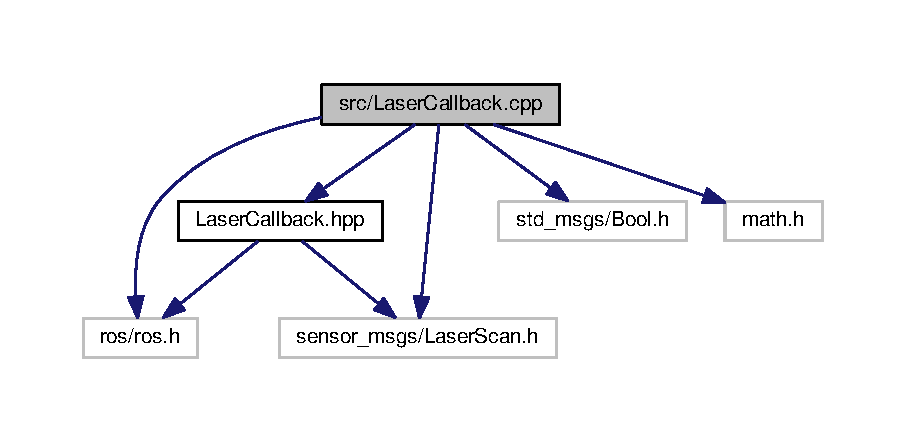
\includegraphics[width=350pt]{LaserCallback_8cpp__incl}
\end{center}
\end{figure}


\subsection{Detailed Description}
The implementation of \hyperlink{classLaserCallback}{Laser\+Callback} class. 


\hypertarget{laserReading_8cpp}{}\section{src/laser\+Reading.cpp File Reference}
\label{laserReading_8cpp}\index{src/laser\+Reading.\+cpp@{src/laser\+Reading.\+cpp}}


This node takes and analyze the range data. Subsequently, pass the the decision made based on the data to the turtle\+Ctrl node which manipulates the turtlebot.  


{\ttfamily \#include \char`\"{}Laser\+Callback.\+hpp\char`\"{}}\\*
{\ttfamily \#include \char`\"{}ros/ros.\+h\char`\"{}}\\*
{\ttfamily \#include \char`\"{}std\+\_\+msgs/\+Bool.\+h\char`\"{}}\\*
{\ttfamily \#include \char`\"{}sensor\+\_\+msgs/\+Laser\+Scan.\+h\char`\"{}}\\*
{\ttfamily \#include \char`\"{}tf/transform\+\_\+listener.\+h\char`\"{}}\\*
{\ttfamily \#include $<$iostream$>$}\\*
{\ttfamily \#include $<$math.\+h$>$}\\*
Include dependency graph for laser\+Reading.\+cpp\+:
\nopagebreak
\begin{figure}[H]
\begin{center}
\leavevmode
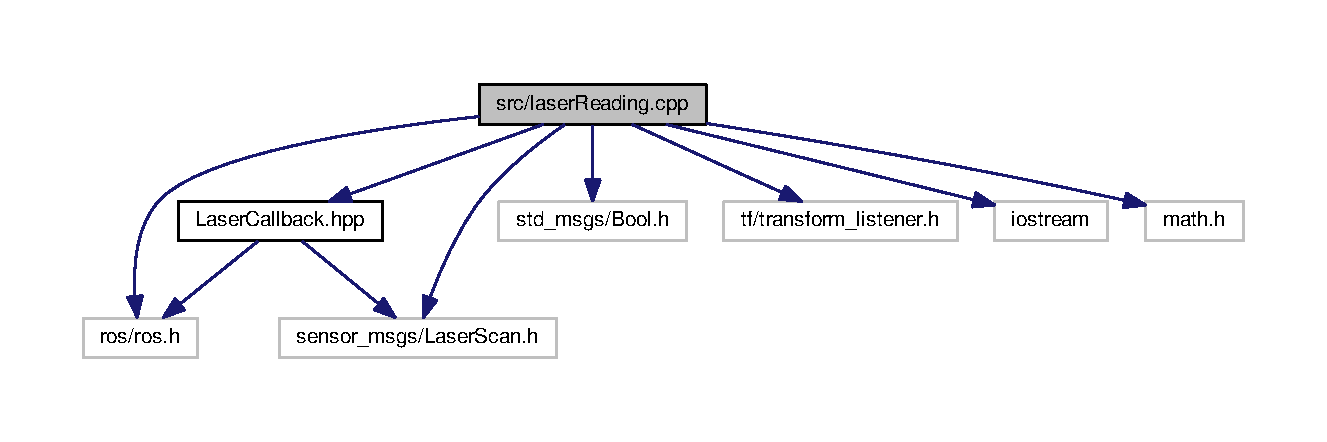
\includegraphics[width=350pt]{laserReading_8cpp__incl}
\end{center}
\end{figure}
\subsection*{Functions}
\begin{DoxyCompactItemize}
\item 
int \hyperlink{laserReading_8cpp_a3c04138a5bfe5d72780bb7e82a18e627}{main} (int argc, char $\ast$$\ast$argv)
\end{DoxyCompactItemize}


\subsection{Detailed Description}
This node takes and analyze the range data. Subsequently, pass the the decision made based on the data to the turtle\+Ctrl node which manipulates the turtlebot. 



\subsection{Function Documentation}
\index{laser\+Reading.\+cpp@{laser\+Reading.\+cpp}!main@{main}}
\index{main@{main}!laser\+Reading.\+cpp@{laser\+Reading.\+cpp}}
\subsubsection[{\texorpdfstring{main(int argc, char $\ast$$\ast$argv)}{main(int argc, char **argv)}}]{\setlength{\rightskip}{0pt plus 5cm}int main (
\begin{DoxyParamCaption}
\item[{int}]{argc, }
\item[{char $\ast$$\ast$}]{argv}
\end{DoxyParamCaption}
)}\hypertarget{laserReading_8cpp_a3c04138a5bfe5d72780bb7e82a18e627}{}\label{laserReading_8cpp_a3c04138a5bfe5d72780bb7e82a18e627}
The ros\+::init() function needs to see argc and argv so that it can perform any R\+OS arguments and name remapping that were provided at the command line. For programmatic remappings you can use a different version of init() which takes remappings directly, but for most command-\/line programs, passing argc and argv is the easiest way to do it. The third argument to init() is the name of the node.

You must call one of the versions of ros\+::init() before using any other part of the R\+OS system.

Node\+Handle is the main access point to communications with the R\+OS system. The first Node\+Handle constructed will fully initialize this node, and the last Node\+Handle destructed will close down the node.

The subscribe() call is how you tell R\+OS that you want to receive messages on a given topic. This invokes a call to the R\+OS master node, which keeps a registry of who is publishing and who is subscribing. Messages are passed to a callback function, here called chatter\+Callback. subscribe() returns a Subscriber object that you must hold on to until you want to unsubscribe. When all copies of the Subscriber object go out of scope, this callback will automatically be unsubscribed from this topic.

The second parameter to the subscribe() function is the size of the message queue. If messages are arriving faster than they are being processed, this is the number of messages that will be buffered up before beginning to throw away the oldest ones.
\hypertarget{turtleCtrl_8cpp}{}\section{src/turtle\+Ctrl.cpp File Reference}
\label{turtleCtrl_8cpp}\index{src/turtle\+Ctrl.\+cpp@{src/turtle\+Ctrl.\+cpp}}


The velocity commanding node. It takes the decision made from the laser\+Reading node and pass the velocities message to the turtlebot.  


{\ttfamily \#include \char`\"{}ros/ros.\+h\char`\"{}}\\*
{\ttfamily \#include \char`\"{}geometry\+\_\+msgs/\+Twist.\+h\char`\"{}}\\*
{\ttfamily \#include \char`\"{}std\+\_\+msgs/\+Bool.\+h\char`\"{}}\\*
{\ttfamily \#include $<$sstream$>$}\\*
{\ttfamily \#include $<$iostream$>$}\\*
Include dependency graph for turtle\+Ctrl.\+cpp\+:
\nopagebreak
\begin{figure}[H]
\begin{center}
\leavevmode
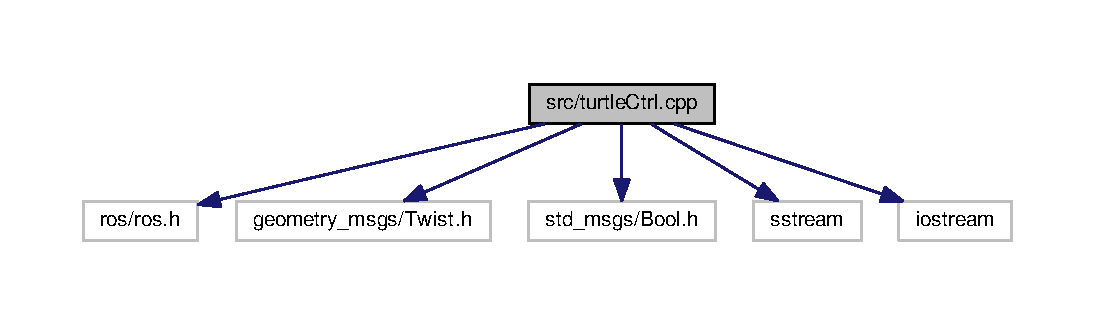
\includegraphics[width=350pt]{turtleCtrl_8cpp__incl}
\end{center}
\end{figure}
\subsection*{Functions}
\begin{DoxyCompactItemize}
\item 
void \hyperlink{turtleCtrl_8cpp_aa5177ba2aaf164b2ff30dcfa8af38b23}{motion\+\_\+callback} (const std\+\_\+msgs\+::\+Bool \&vel\+\_\+msg)
\item 
int \hyperlink{turtleCtrl_8cpp_a3c04138a5bfe5d72780bb7e82a18e627}{main} (int argc, char $\ast$$\ast$argv)
\end{DoxyCompactItemize}
\subsection*{Variables}
\begin{DoxyCompactItemize}
\item 
geometry\+\_\+msgs\+::\+Twist \hyperlink{turtleCtrl_8cpp_aba2f97176e275688941f5c2a40324b8a}{msg}
\end{DoxyCompactItemize}


\subsection{Detailed Description}
The velocity commanding node. It takes the decision made from the laser\+Reading node and pass the velocities message to the turtlebot. 



\subsection{Function Documentation}
\index{turtle\+Ctrl.\+cpp@{turtle\+Ctrl.\+cpp}!main@{main}}
\index{main@{main}!turtle\+Ctrl.\+cpp@{turtle\+Ctrl.\+cpp}}
\subsubsection[{\texorpdfstring{main(int argc, char $\ast$$\ast$argv)}{main(int argc, char **argv)}}]{\setlength{\rightskip}{0pt plus 5cm}int main (
\begin{DoxyParamCaption}
\item[{int}]{argc, }
\item[{char $\ast$$\ast$}]{argv}
\end{DoxyParamCaption}
)}\hypertarget{turtleCtrl_8cpp_a3c04138a5bfe5d72780bb7e82a18e627}{}\label{turtleCtrl_8cpp_a3c04138a5bfe5d72780bb7e82a18e627}
This tutorial demonstrates simple sending of messages over the R\+OS system. The ros\+::init() function needs to see argc and argv so that it can perform any R\+OS arguments and name remapping that were provided at the command line. For programmatic remappings you can use a different version of init() which takes remappings directly, but for most command-\/line programs, passing argc and argv is the easiest way to do it. The third argument to init() is the name of the node.

You must call one of the versions of ros\+::init() before using any other part of the R\+OS system.

Node\+Handle is the main access point to communications with the R\+OS system. The first Node\+Handle constructed will fully initialize this node, and the last Node\+Handle destructed will close down the node.

The advertise() function is how you tell R\+OS that you want to publish on a given topic name. This invokes a call to the R\+OS master node, which keeps a registry of who is publishing and who is subscribing. After this advertise() call is made, the master node will notify anyone who is trying to subscribe to this topic name, and they will in turn negotiate a peer-\/to-\/peer connection with this node. advertise() returns a Publisher object which allows you to publish messages on that topic through a call to publish(). Once all copies of the returned Publisher object are destroyed, the topic will be automatically unadvertised.

The second parameter to advertise() is the size of the message queue used for publishing messages. If messages are published more quickly than we can send them, the number here specifies how many messages to buffer up before throwing some away.

A subscribing node that reads the motion mode from the laser\+Reading node. Based on its value, turtle\+Ctrl would decide the states (velocities) of of the turtlebot.

A count of how many messages we have sent. This is used to create a unique string for each message.

The publish() function is how you send messages. The parameter is the message object. The type of this object must agree with the type given as a template parameter to the advertise$<$$>$() call, as was done in the constructor above.\index{turtle\+Ctrl.\+cpp@{turtle\+Ctrl.\+cpp}!motion\+\_\+callback@{motion\+\_\+callback}}
\index{motion\+\_\+callback@{motion\+\_\+callback}!turtle\+Ctrl.\+cpp@{turtle\+Ctrl.\+cpp}}
\subsubsection[{\texorpdfstring{motion\+\_\+callback(const std\+\_\+msgs\+::\+Bool \&vel\+\_\+msg)}{motion_callback(const std_msgs::Bool &vel_msg)}}]{\setlength{\rightskip}{0pt plus 5cm}void motion\+\_\+callback (
\begin{DoxyParamCaption}
\item[{const std\+\_\+msgs\+::\+Bool \&}]{vel\+\_\+msg}
\end{DoxyParamCaption}
)}\hypertarget{turtleCtrl_8cpp_aa5177ba2aaf164b2ff30dcfa8af38b23}{}\label{turtleCtrl_8cpp_aa5177ba2aaf164b2ff30dcfa8af38b23}
Takes the msg from the laser\+Reading node and decides the velocities of the turtlebot. 

\subsection{Variable Documentation}
\index{turtle\+Ctrl.\+cpp@{turtle\+Ctrl.\+cpp}!msg@{msg}}
\index{msg@{msg}!turtle\+Ctrl.\+cpp@{turtle\+Ctrl.\+cpp}}
\subsubsection[{\texorpdfstring{msg}{msg}}]{\setlength{\rightskip}{0pt plus 5cm}geometry\+\_\+msgs\+::\+Twist msg}\hypertarget{turtleCtrl_8cpp_aba2f97176e275688941f5c2a40324b8a}{}\label{turtleCtrl_8cpp_aba2f97176e275688941f5c2a40324b8a}
The geometry msgs that would be sent to the mobile node 
%--- End generated contents ---

% Index
\backmatter
\newpage
\phantomsection
\clearemptydoublepage
\addcontentsline{toc}{chapter}{Index}
\printindex

\end{document}
